% Options for packages loaded elsewhere
\PassOptionsToPackage{unicode}{hyperref}
\PassOptionsToPackage{hyphens}{url}
%
\documentclass[
  11pt,
]{article}
\usepackage{amsmath,amssymb}
\usepackage{lmodern}
\usepackage{ifxetex,ifluatex}
\ifnum 0\ifxetex 1\fi\ifluatex 1\fi=0 % if pdftex
  \usepackage[T1]{fontenc}
  \usepackage[utf8]{inputenc}
  \usepackage{textcomp} % provide euro and other symbols
\else % if luatex or xetex
  \usepackage{unicode-math}
  \defaultfontfeatures{Scale=MatchLowercase}
  \defaultfontfeatures[\rmfamily]{Ligatures=TeX,Scale=1}
\fi
% Use upquote if available, for straight quotes in verbatim environments
\IfFileExists{upquote.sty}{\usepackage{upquote}}{}
\IfFileExists{microtype.sty}{% use microtype if available
  \usepackage[]{microtype}
  \UseMicrotypeSet[protrusion]{basicmath} % disable protrusion for tt fonts
}{}
\makeatletter
\@ifundefined{KOMAClassName}{% if non-KOMA class
  \IfFileExists{parskip.sty}{%
    \usepackage{parskip}
  }{% else
    \setlength{\parindent}{0pt}
    \setlength{\parskip}{6pt plus 2pt minus 1pt}}
}{% if KOMA class
  \KOMAoptions{parskip=half}}
\makeatother
\usepackage{xcolor}
\IfFileExists{xurl.sty}{\usepackage{xurl}}{} % add URL line breaks if available
\IfFileExists{bookmark.sty}{\usepackage{bookmark}}{\usepackage{hyperref}}
\hypersetup{
  pdftitle={Estimating survival in left filtered data},
  pdfauthor={Kevin Chen},
  hidelinks,
  pdfcreator={LaTeX via pandoc}}
\urlstyle{same} % disable monospaced font for URLs
\usepackage[margin=2.54cm]{geometry}
\usepackage{graphicx}
\makeatletter
\def\maxwidth{\ifdim\Gin@nat@width>\linewidth\linewidth\else\Gin@nat@width\fi}
\def\maxheight{\ifdim\Gin@nat@height>\textheight\textheight\else\Gin@nat@height\fi}
\makeatother
% Scale images if necessary, so that they will not overflow the page
% margins by default, and it is still possible to overwrite the defaults
% using explicit options in \includegraphics[width, height, ...]{}
\setkeys{Gin}{width=\maxwidth,height=\maxheight,keepaspectratio}
% Set default figure placement to htbp
\makeatletter
\def\fps@figure{htbp}
\makeatother
\setlength{\emergencystretch}{3em} % prevent overfull lines
\providecommand{\tightlist}{%
  \setlength{\itemsep}{0pt}\setlength{\parskip}{0pt}}
\setcounter{secnumdepth}{-\maxdimen} % remove section numbering
\PassOptionsToPackage{no-math}{fontspec}

%---------------------------------------------------------------------------
% Kevin's style file
%---------------------------------------------------------------------------
\usepackage{ifxetex,ifluatex}

%---------------------------------------------------------------------------
% General
%---------------------------------------------------------------------------

% When testing
% \usepackage{lipsum}

% Line numbering
\usepackage{lineno}

% Usage
	% \linenumbers
	% \modulolinenumbers[2]
	% \renewcommand\thelinenumber{\color{red}\Roman{linenumber}}
	% \begin{linenumbers}  \end{linenumbers}


\usepackage{setspace}
%\doublespacing


\usepackage{outlines}
% \usepackage{enumerate}
\usepackage{enumitem} % more powerful than enumerate
% \setenumerate[4]{label=\alph*).}

\setlength\parindent{0pt} % Removes all indentation from paragraphs

\usepackage{sectsty} % Allows customizing section commands
% \renewcommand{\thesection}{\Alph{section}} % Lettered, not numbered sections
% \allsectionsfont{\centering \normalfont\scshape} % Make all sections centered, the default font and small caps
%\numberwithin{equation}{section} % Number equations within sections
%\numberwithin{figure}{section} % Number figures within sections
%\numberwithin{table}{section} % Number tables within sections

\usepackage{multicol}
\setlength{\columnsep}{15pt}
\newlength\Colsep

%---------------------------------------------------------------------------
% Tables, figures, images
%---------------------------------------------------------------------------
\usepackage{color}
% \usepackage[usenames,dvipsnames]{xcolor}
\usepackage{xparse}
\usepackage{xhfill}
\ifnum 0\ifxetex 1\fi\ifluatex 1\fi=0
% Requires pdfTeX
\usepackage{linegoal}
\fi

\usepackage{longtable}
\setlength{\LTcapwidth}{\textwidth}
\usepackage{xtab, booktabs}
\usepackage{multirow}
\usepackage[flushleft]{threeparttable} % Suzanne's

\usepackage{float} % Check code chunks section for floatrow

\usepackage{graphicx}
% \usepackage{grffile}
% \usepackage{subcaption}
% For tables and figures in parts %%%%
\usepackage{caption}
% \DeclareCaptionLabelFormat{cont}{#1~#2\alph{ContinuedFloat}}
% \captionsetup[ContinuedFloat]{labelformat=cont}
%\graphicspath{ {file.path.here} }

% Set column widths in tabular environment!
\usepackage{array}
\newcommand{\PreserveBackslash}[1]{\let\temp=\\#1\let\\=\temp}
\newcolumntype{C}[1]{>{\PreserveBackslash\centering}p{#1}}
\newcolumntype{R}[1]{>{\PreserveBackslash\raggedleft}p{#1}}
\newcolumntype{L}[1]{>{\PreserveBackslash\raggedright}p{#1}}

% STATA output for `estout` package
\def\sym#1{\ifmmode^{#1}\else\(^{#1}\)\fi}

%---------------------------------------------------------------------------
% Header/footer
%---------------------------------------------------------------------------
\usepackage{fancyhdr}
\pagestyle{fancyplain}
\fancyhead[L]{}
\fancyhead[C]{}
\fancyhead[R]{}
% \fancyfoot[L]{}
% \fancyfoot[C]{}
% \fancyfoot[R]{\thepage}
\renewcommand{\headrulewidth}{0pt}
% \renewcommand{\footrulewidth}{0pt}
\setlength{\headheight}{14.5pt}

%---------------------------------------------------------------------------
% Supplement (compatible for Beamer and Article)
%---------------------------------------------------------------------------
\input{\string~/HeadRs/common_supplement.tex}

%---------------------------------------------------------------------------
% Bibliography
%---------------------------------------------------------------------------
% \usepackage[backend=bibtex]{biblatex}

%---------------------------------------------------------------------------
% Usage
%---------------------------------------------------------------------------

% For use in LaTex or Sweave:
% \input{/Users/kevinchen/Documents/computing/HeadRs/StatHead.tex}

% An example YAML header for Rmd
% ---
% title: "Stat 2"
% author: "Kevin Chen"
% date: \today
% output:
%   pdf_document:
%      # keep_tex: true
%     #  pandoc_args: [
%     #   "-V", "classoption=twocolumn"
%     # ]
%      includes:
%         in_header: /Users/kevinchen/Documents/computing/HeadRs/StatHead.tex
% bibliography: /Users/kevinchen/Documents/2017 Fa/245/MV_FinalProj/mv_final.bib
% csl: /Users/kevinchen/Documents/computing/HeadRs/AMA.csl
% geometry: margin=2cm, bottom=2.5cm
% ---


%---------------------------------------------------------------------------
% Fonts
%---------------------------------------------------------------------------

%\usepackage[T1]{fontenc} % Use 8-bit encoding that has 256 glyphs
%\usepackage[utf8]{inputenc}
% Latin Modern Roman
% \usepackage{lmodern}
%\usepackage{fourier} % Use the Adobe Utopia font for the document - comment this line to return to the LaTeX default

\ifluatex
%%%%%%%%%%%%%%%%%%%%%%%%%%%
% For Arial (with lualatex)
%%%%%%%%%%%%%%%%%%%%%%%%%%%
\usepackage[no-math]{fontspec}
% \setmainfont{Arial}[
% % Options below necessary for Windows
% 	% Extension = .ttf,
% 	% UprightFont = *,
% 	% BoldFont = *bd,
% 	% ItalicFont = *i,
% 	% BoldItalicFont = *bi
% 	]
% In YAML
% ---
% mainfont: Arial
% ---
% \usepackage{lualatex-math}

% Math as text, but numerals do not mpa well becuase
% mathastext clahes with unicode-math
% \usepackage[italic]{mathastext}
%%%%%%%%%%%%%%%%%%%%%%%%%%%
\fi
\ifluatex
  \usepackage{selnolig}  % disable illegal ligatures
\fi
\newlength{\cslhangindent}
\setlength{\cslhangindent}{1.5em}
\newlength{\csllabelwidth}
\setlength{\csllabelwidth}{3em}
\newenvironment{CSLReferences}[2] % #1 hanging-ident, #2 entry spacing
 {% don't indent paragraphs
  \setlength{\parindent}{0pt}
  % turn on hanging indent if param 1 is 1
  \ifodd #1 \everypar{\setlength{\hangindent}{\cslhangindent}}\ignorespaces\fi
  % set entry spacing
  \ifnum #2 > 0
  \setlength{\parskip}{#2\baselineskip}
  \fi
 }%
 {}
\usepackage{calc}
\newcommand{\CSLBlock}[1]{#1\hfill\break}
\newcommand{\CSLLeftMargin}[1]{\parbox[t]{\csllabelwidth}{#1}}
\newcommand{\CSLRightInline}[1]{\parbox[t]{\linewidth - \csllabelwidth}{#1}\break}
\newcommand{\CSLIndent}[1]{\hspace{\cslhangindent}#1}

\title{Estimating survival in left filtered data}
\author{Kevin Chen}
\date{Stat 256: Causal Inference (Fall 2021)}

\begin{document}
\maketitle

\fancyhead[R]{Kevin Chen}
\fancyhead[L]{}
\renewcommand{\headrulewidth}{0pt}

\onehalfspacing
\renewcommand{\arraystretch}{1.1}

\thispagestyle{empty}

\setlength{\columnseprule}{0pt}

\hypertarget{introduction}{%
\section{Introduction}\label{introduction}}

The United Auto Workers-General Motors (UAW-GM) Cohort Study is a
longitudinal occupational cohort study established in the early 1980s to
study the health effects of metalworking fluids (Eisen et al. 1992,
2001). Metalworking fluids (MWF) are complex mixtures of fluids used in
industrial metalworking operations to lubricate and cool machinery and
parts. The three major classes of MWF are straight, soluble, and
synthetic metalworking fluids (Byers 2006). Possible routes of human
exposure include absorption through skin, inhalation of aerosols, and
ingestion of droplets.

A central concern in the analysis of longitudinal occupational cohort
data is the potential for bias due to the healthy worker survivor effect
(HWSE), the phenomenon by which healthy individuals remain at work,
while less healthy individuals leave work -- possibly in response to
exposure-related health decline. In the presence of the HWSE, those with
the highest cumulative occupational exposures are also those who are
less at risk of disease (more likely to have potential outcome no
disease under both exposure and no exposure scenarios). Thus, standard
measures of association would show an inverse relationship between
occupational exposure and poor health outcomes (Arrighi and
Hertz-Picciotto 1994). The HWSE is an example of time-varying
confounding affected by past exposure. Previous studies have attempted
to assess the presence of the HWSE in observed data by assessing
so-called path-specific associations using Cox proportional hazards
modeling (Naimi et al. 2013; Garcia et al. 2017). However, in those
studies, the estimates were themselves subject to the confounding
structures they sought to characterize.

If conditional sequential ignorability of exposure and censoring status
at each point in follow-up and positivity (overlap) can be attained
given covariate history, then longitudinal causal methods can be applied
to account for the HWSE. Past studies have applied causal methods
capable of accounting for time-varying confounding affected by past
exposure to the study of MWF exposures and cancer mortality outcomes in
the UAW-GM Cohort Study (Garcia et al. 2018; Izano et al. 2019).
However, the study of cancer incidence outcomes is further problematized
by the incomplete observation of cancer incidence outcomes at every
point of follow-up over the study period. Nonetheless, we wish to make
inferences about the carcinogenicity of MWF exposure over an
individual's lifetime starting upon entry into the workforce. The UAW-GM
Cohort included those hired roughly between 1938 and 1985. However,
cancer incidence reporting did not begin until 1973. Hence, our observed
cohort data exhibits \emph{left filtering}: cancer incidence is the
outcome of interest, but before 1985, both cancer incidence status and
time of cancer incidence are unknown. Observation of the complete cancer
incidence outcome vector over the study period was conditional on an
individual surviving to 1985 cancer-free.

In the presence of the HWSE, left filtering implies outcome
misclassification that is informative of true cancer status. As part of
her dissertation research, Izano (2017) conducted a quantitative bias
analysis for the estimation of survival curves using left filtered data
in the presence of HWSE. She simulated data compatible with the HWSE and
estimated cancer-free survival curves using an inverse probability of
treatment and censoring weighted Kaplan-Meier (WKM) estimator and the
WKM with an Aalen filter for left-filtering (AWKM) (Andersen et al.
1993; Xie and Liu 2005). Data were simulated under five different
scenarios. The survival curves under the following interventions were
computed or estimated in 250 replicates: (1) always exposed at work with
no censoring due to death and (2) never exposed at work with no
censoring due to death. For each intervention, three survival curves
were produced: (1) the true survival curve, (2) the WKM survival curve,
and (3) AWKM survival curve. Estimator bias was evaluated by comparing
the average of 250 estimates of to the average difference in cancer-free
survival under the two rules to the true average difference in survival
when exposure and censoring were controlled deterministically.

The present project replicates the simulation and bias analyses
presented in Chapter 3 of Izano (2017), embeds the problem in the
non-parametric structural causal approach of Pearl (1995), and applies
the WKM and AWKM estimators to the estimation of digestive-system
cancer-free survival under exposure and no censoring rules in the UAW-GM
Cohort. The \texttt{stremr} package was used to estimate the WKM and
AWKM survival curves in both the simulation and the applied analyses
(Sofrygin, van der Laan, and Neugebauer 2021). All code necessary for
replicating the analyses presented here may be found on
\href{https://github.com/kvntchn/gm-delayed-entry.git}{GitHub/kvntchn/gm-delayed-entry}.
Note that running the script for the applied analyses will require
additional permissions.

\hypertarget{methods}{%
\section{Methods}\label{methods}}

\hypertarget{causal-model}{%
\subsection{Causal model}\label{causal-model}}

The UAW-GM Cohort data included person-year level exposure, outcome, and
covariate data starting at hire. To emulate the shape of the data for
this longitudinal cohort, we considered 20 years of data over time
indexed by years since hire. Notation representing the variables of
interest are presented in Table \ref{tab:variables}. The causal model
represents hypothetical relationships between variables over time
compatible with the theory underlying the HWSE in longitudinal
occupational cohort studies. At each time point, the effect of
cumulative exposure \(\bar A(t)\) on cancer incidence \(Y^*(t)\) is
confounded by the path through employment status \(N(t)\) and underlying
health \(H(t)\) as well as the path through past exposure
\(\bar A(t - 1)\) and vital status \(D(t)\). These paths follow
straightforward logic: occupational exposure depends upon employment
status and past exposure; mortality status is affected by past exposure
and cancer history. Confounding by baseline covariates \(W\) is assumed
throughout.

\begin{table}
\caption{Descriptions of variables.}\label{tab:variables}
\begin{center}
\begin{tabular}{lp{0.5\linewidth}}
\toprule
 Variable  &  Description                                 \\ \midrule
 $R$       & Time until start of registry \\
 $W$       & Baseline covariates \\
 $S$       & Susceptibility to effects of metalworking fluid exposure \\
 $H(t)$    & Adverse health status at time $t$ \\
 $N(t)$    & Employment status at time $t$ \\
 $A(t)$    & Metalworking fluid exposure at time $t$ \\
 $D(t)$    & Mortality status at time $t$ \\
 $Y^*(t)$  & Cancer status at time $t$ \\
 $Y(t)$    & Observed Cancer status at time $t$ \\
 $t = \{1, 2, \ldots, 20\}$ & Time, indexed in years after hire \\
 \bottomrule
\end{tabular}
\end{center}\end{table}

Assume we have \(n = 50\,000\) iid units in \(X\) with
\[X_i(t) = \left(R_i = 0, W_i, S_i, \bar H_i(t), \bar N_i(t), \bar A_i(t), \bar a_i(t), \bar Y^*_i(t) = \bar Y_i(t) \right).\]
In general, we use bar notation to indicate variable history as follows
\(\bar X_i(t) = \left(X_i(k)\right)_{k = 1}^t\). Note that true cancer
status \(Y^*(t)\) is not observed until \(t \ge R\), after the start of
the registry. Call \(X\) the full data, where we have \(R = 0\) for all.
In the observed data \(X^\text{obs}\), we cannot assume \(R = 0\) for
all. Additionally, susceptibility \(S\) and underlying health status
\(H\) are not known:
\[X^\text{obs}_i(t) = \left(R_i, W_i, \bar N_i(t), \bar A_i(t), \bar a_i(t), \bar Y_i(t) \right).\]
Under the causal model, we assume the following non-parametric
structural equations: \[\begin{aligned}
R     & = f_R \left( U_R \right) \\
W     & = f_W \left( U_W \right) \\
S     & = f_S \left( U_S \right) \\
H(t)  & = f_{H(t)} \left( H(t - 1), U_{H(t)} \right) \\
N(t)  & = f_{N(t)} \left( W, N(t - 1), H(t), A(t - 1), U_{N(t)} \right) \\
A(t)  & = f_{A(t)} \left( W, \bar A(t - 1), N(t), U_{A(t)} \right) \\
D(t)  & = f_{D(t)} \left( W, \bar A(t - 1), D(t - 1), Y^*(t - 1), U_{D(t)} \right) \\
Y^*(t)& = f_{Y^*(t)} \left(W, S, H(t), \bar A (t), D(t), Y^*(t - 1), U_{Y^*(t)} \right) \\
Y(t) & = Y^*(t) \times \Ind{Y^*(\lfloor R \rfloor) = 0} \times \Ind{D(t) = 0} \ .
\end{aligned}\] The exogenous variables (errors)
\(U = \left( U_R, U_W, U_S, U_{H(t)}, U_{N(t)}, U_{A(t)}, U_{D(t)}, U_{Y^*(t)} \right)_{t = 1}^{T}\)
are mutually independent. Exposure status is a time-varying indicator,
and exposure history is summarized as
\(\bar A(t) = \Ind{\sum_{k = 1}^t\Ind{A(k) = 1} > 0}\). The outcome of
interest is a survival outcome, so
\(Y^*(t - 1) = 1 \Rightarrow Y^*(t) = 1\). The observed outcome \(Y(t)\)
at time \(t\) is a function of true outcome status, time of left
censoring, and time of right censoring. An abbreviated directed acyclic
graph (DAG) representing the causal relationships encoded in the
equations above is presented in Figure \ref{fig:dag}.

\begin{figure}
\caption{Directed acyclic graph representing the causal relationships encoded in the non-parametric structural equation model at time $t$.}
\label{fig:dag}
\begin{center}
\begin{tikzpicture}[>= stealth, auto, node distance = 2.25cm, semithick, fill=white, inner sep=0pt]
\tikzstyle{every state}=[shape = circle, align = center, draw = none]
\node[state] (H0) {$H(t - 1)$};
\node[state] (N0) [below right of=H0] {$N(t - 1)$};
\node[state] (A0) [below right of=N0] {$\bar A(t - 1)$};
\node[state] (D0) [below right of=A0] {$D(t - 1)$};
\node[state] (Y0) [below right of=D0] {$Y^*(t - 1)$};
\node[state] (W) [above right of=H0] {$W$};
\node[state] (H) [right of=H0, node distance = 4cm] {$H(t)$};
\node[state] (N) [below right of=H, node distance = 4cm] {$N(t)$};
\node[state] (A) [below right of=N, node distance = 4cm] {$\bar A(t)$};
\node[state] (D) [above right of=N, node distance = 3cm] {$D(t)$};
\node[state] (Y) [above right of=A, node distance = 3cm] {$Y^*(t)$};
\node[state] (S) [above right of=D, node distance = 3cm] {$S$};
%
\path[->] (H0) edge (N0);
\path[->] (N0) edge (A0);
\path[->] (A0) edge [bend right=30] (Y0);
\path[->] (H0) edge (H);
\path[->] (W) edge [bend right=10] (N);
\path[->] (N0) edge (N);
\path[->] (H) edge (N);
\path[->] (A0) edge (N);
\path[->] (W) edge [bend right=15] (A);
\path[->] (A0) edge (A);
\path[->] (N) edge (A);
\path[->] (W) edge (D);
\path[->] (A0) edge [bend left=15] (D);
\path[->] (D0) edge [bend right=15] (D);
\path[->] (Y0) edge [bend right=10] (D);
\path[->] (W) edge [bend left=5] (Y);
\path[->] (S) edge [bend left=30] (Y);
\path[->] (S) edge [bend left=15] (Y0);
\path[->] (H) edge (Y);
\path[->] (A) edge (Y);
\path[->] (D) edge (Y);
\path[->] (Y0) edge (Y);
\end{tikzpicture}
\end{center}
\end{figure}

Figure \ref{fig:dag} clarifies our conceptualization of the HWSE. At
each time point \(t\), the cumulative effect of exposure \(\bar A(t)\)
on cancer incidence \(Y^*(t)\) is confounded by employment status
\(N(t)\) through the backdoor path
\(\bar A(t) \leftarrow N(t) \leftarrow H(t) \rightarrow Y^*(t)\). In the
absence of observed data on health status \(H(t)\), an analyst may be
tempted to conduct an analysis by simply ``blocking'' or conditioning on
employment status \(N(t)\), but doing so would introduce collider bias
while blocking the causal path between past exposure \(\bar A(t - 1)\)
and cancer \(Y^*(t)\). Furthermore, an analysis starting at an arbitrary
time point after the time origin (hire) would be tantamount to
conditioning on those still alive at that time, which would result in
both collider bias and the conditioning on nodes on the causal path
between the exposure and the outcome of interest.

\hypertarget{simulation}{%
\subsection{Simulation}\label{simulation}}

To generate data compatible with our structural causal model, we imposed
parametric relationships between the variables. For the \(n = 50\,000\)
units over \(T = 20\) years, we have:

\begin{itemize}
\tightlist
\item
  \(U_j \overset{\text{iid}}{\sim} \text{uniform}\,[0,1]\) for all \(j\)
\item
  In full data \(R = 0\) otherwise \(R \sim \text{uniform}\,[0, 30]\)
\item
  \(W = \Ind{U_W \le p_W} \sim \text{Bernoulli}\left( p_W \right)\)
\item
  \(S = \Ind{U_S \le p_S} \sim \text{Bernoulli}\,(p_S)\)
\item
  If \(H(t - 1) = 1\), then \(H(t) = 1\) otherwise
  \(H(t) = \Ind{U_{H(t)} \le p_H} \sim \text{Bernoulli}\,(p_H)\)
\item
  if \(N(t - 1) = 0\) then \(N(t) = 0\) otherwise
  \[N(t) \sim \text{Bernoulli}\left\{
    \text{logit}\,\left(
        \beta_0^N
        + \beta_W^N W
        + \beta_H^N H(t)
        + \beta_A^N A(t - 1) \times \Ind{t > 1}
        + U_{N(t)}
    \right)
    \right\}\]
\item
  If \(N(t) = 0\) then \(A(t) = 0\) otherwise
  \[A(t) \sim \text{Bernoulli}\left\{
    \text{logit}\,\left(
        \left( \beta_0^A + \beta_W^A W\right) \times \Ind{t = 1}
        + \beta_A^A A(t - 1) \times \Ind{t > 1}
        + U_{A(t)}
    \right)
    \right\}\]
\item
  If \(D(t - 1) = 1\) then \(D(t) = 1\) otherwise
  \[D(t) \sim \text{Bernoulli}\left\{
    \text{logit}\,\left(\begin{aligned}
        \beta_0^D
        + \beta_W^D W
        + \beta_{\bar A}^D \bar A(t - 1) \times \Ind{t > 1} \\
        + \beta_{\bar Y}^D \sum_{k = 1}^{t - 1} Y^*(k) \times \Ind{t > 1}
        + U_{D(t)}
    \end{aligned}\right)
    \right\}\]
\item
  If \(Y^*(t - 1) = 1\) then \(Y^*(t) = 1\) otherwise
  \[Y^*(t) \sim \text{Bernoulli}\left\{
    \text{logit}\,\left(\begin{aligned}
        \beta_0^Y
        + \beta_W^Y W
        + \beta_{A}^Y A(t)
        + \beta_{\bar A}^Y \bar A(t - 1) \times \Ind{t > 1} \\
        + \beta_{S}^Y S \times \bar A(t)
        + \beta_{H}^Y H(t)
        + U_{Y^*(t)}
    \end{aligned}\right)
    \right\}\]
\item
  If \(t < R\) then \(Y(t) = 0\)
\item
  If \(t \ge R\) then
  \(Y(t) = Y^*(t) \times \Ind{Y^*(\lfloor R \rfloor) = 0} \times \Ind{D(t) = 0}\).
\end{itemize}

Five sets of data were generated using these equations, but with
different parameters, to represent five scenarios. Scenario 1 represents
the base case where 10\% of workers are susceptible to exposure-related
effects, the odds ratio of mortality each additional year following
cancer diagnosis is about 1.6, and there is moderate time-varying
confounding by health status. In scenario 2, we have greater
cancer-related mortality by increasing \(\beta_{\bar Y}^D\). In scenario
3, we increase \(p_S\), the proportion of the study population
susceptible to the carcinogenic effects of MWF exposure. In scenario 4,
we consider greater time-varying confounding by health status by
increasing \(\beta_H^N\) and \(\beta_H^Y\). In the last scenario, we
have greater background cancer incidence by increasing \(\beta_0^Y\).
The sets of parameters used in the five scenarios are presented in Table
\ref{tab:params}.

\begin{table}[h]
\caption{Simulation parameters.}
\label{tab:params}
\begin{center}
\begin{tabular}{rrrrrr}
  \toprule
Parameter & Scenario 1 & Scenario 2 & Scenario 3 & Scenario 4 & Scenario 5 \\ 
  \midrule
$p_S$ & 0.10 & 0.10 & \textbf{0.20} & 0.10 & 0.10 \\ 
  $p_W$ & 0.20 & 0.20 & 0.20 & 0.20 & 0.20 \\ 
  $p_H$ & 0.30 & 0.30 & 0.30 & 0.30 & 0.30 \\ 
  $\beta_0^N$ & 3.00 & 3.00 & 3.00 & 3.00 & 3.00 \\ 
  $\beta_W^N$ & -0.10 & -0.10 & -0.10 & -0.10 & -0.10 \\ 
  $\beta_H^N$ & -0.50 & -0.50 & -0.50 & \textbf{-1.50} & -0.50 \\ 
  $\beta_A^N$ & -1.50 & -1.50 & -1.50 & -1.50 & -1.50 \\ 
  $\beta_0^A$ & -1.50 & -1.50 & -1.50 & -1.50 & -1.50 \\ 
  $\beta_W^A$ & -0.50 & -0.50 & -0.50 & -0.50 & -0.50 \\ 
  $\beta_A^A$ & 2.50 & 2.50 & 2.50 & 2.50 & 2.50 \\ 
  $\beta_0^D$ & -5.50 & -5.50 & -5.50 & -5.50 & -5.50 \\ 
  $\beta_W^D$ & 1.00 & 1.00 & 1.00 & 1.00 & 1.00 \\ 
  $\beta_{\bar A}^D$ & 0.50 & 0.50 & 0.50 & 0.50 & 0.50 \\ 
  $\beta_{\bar Y}^D$ & 0.50 & \textbf{2.00} & 0.50 & 0.50 & 0.50 \\ 
  $\beta_0^Y$ & -7.00 & -7.00 & -7.00 & -7.00 & \textbf{-6.00} \\ 
  $\beta_W^Y$ & 2.00 & 2.00 & 2.00 & 2.00 & 2.00 \\ 
  $\beta_A^Y$ & 0.25 & 0.25 & 0.25 & 0.25 & 0.25 \\ 
  $\beta_{\bar A}^Y$ & 0.20 & 0.20 & 0.20 & 0.20 & 0.20 \\ 
  $\beta_H^Y$ & 0.70 & 0.70 & 0.70 & \textbf{1.70} & 0.70 \\ 
  $\beta_S^Y$ & 0.30 & 0.30 & 0.30 & 0.30 & 0.30 \\ 
   \bottomrule
\end{tabular}
\end{center}
\end{table}

\hypertarget{interventions-potential-outcomes-target-parameters-and-estimation}{%
\subsection{Interventions, potential outcomes, target parameters, and
estimation}\label{interventions-potential-outcomes-target-parameters-and-estimation}}

The substantive question of interest was the causal effect of
occupational exposure to MWF on cancer incidence risk. Since
occupational MWF exposure occurs only when individuals are at work, we
defined dynamic exposure regimes that depend on employment status. Under
rule \(a_0\), set \(D(t) = 0\), and set \(A(t) = 0\) while \(N(t) = 1\).
Under rule \(a_1\), set \(D(t) = 0\), and set \(A(t) = 1\) while
\(N(t) = 1\). Under both rules, we prevented censoring by death as if it
were intervenable. The causal effect was defined by contrasting the
survival functions \(S_{a_1}(t) = 1 - \E{Y_{a_1}(t)}\) under rule
\(a_1\) to \(S_{a_0}(t) = 1 - \E{Y_{a_0}(t)}\) that under rule \(a_0\).
Note that this causal estimand was defined over \emph{a priori
counterfactuals} not observable in the real world (Frangakis and Rubin
2002). This approach is standard in epidemiologic studies.

The survival function expresses the probability that a person following
rule \(a\) is cancer-free at the end of time point \(t\). The expected
time until cancer under rule \(a\) is
\(\mu_{a} = \sum_0^K S_{a}(t) \, dt\). The parameter used in the
estimation of bias was the summary measure
\(\psi = \mu_{a_1} - \mu_{a_0}\), the difference in expected time until
event under two different interventions over 20 years of follow-up under
five different data generating scenarios. Bias was evaluated by
comparing estimates of \(\psi\) to its true value in 250 simulations per
scenario (the original analysis performed 500). The true value was
calculated by simulating the full data for \(500\,000\) individuals (the
original analysis used one million) with rules \(a_0\) and \(a_1\)
applied deterministically. Estimates of \(\psi\) were obtained by
estimating the survival curves \(S_a(t)\) using two estimators: the
inverse probability weighted Kaplan-Meier estimator (WKM) and the
Aalen-filtered WKM (AWKM). These survival estimators are detailed in the
following section.

\hypertarget{kaplan-meier-estimator-and-extensions}{%
\subsection{Kaplan-Meier estimator and
extensions}\label{kaplan-meier-estimator-and-extensions}}

To estimate survival, we applied extensions of the widely-known
Kaplan-Meier (KM) estimator for survival (Kaplan and Meier 1958). First,
we review the estimator of Xie and Liu (2005), an extension of the KM
estimator where units are weighted by the inverse probability of
treatment. The standard KM estimator requires counting up the number of
cases \(c^0_{a}(t)\) that occurred in interval \((t - 1, t]\) and the
number of units at risk \(r^0_{a}(t)\) in that interval at all event
times \(t\). Assuming cancer status was assessed at the end of regular
intervals \(t = 1, \ldots, K\), we have: \[\begin{aligned}
c^0_{a} (t)
& = \sum_i^n \Ind{Y_i(t) = 1} \times \Ind{Y_i(t - 1) = 0} \times \Ind{\bar A_i (t) = \bar a(t)} \\
r^0_{a} (t)
& = \sum_i^n \Ind{Y_i(t - 1) = 0} \times \Ind{\bar A_i (t) = \bar a(t)}.
\end{aligned}\] The standard survival estimator is \[\hat S^0_{a}(t) =
\begin{cases}
1 & \text{if } t < t_1 \\
\prod_{j \le t} \left(1 - \frac{c^0_{a}(j)}{r^0_{a}(j)}\right) & \text{if } t \ge t_1 \\
\end{cases}\] where \(t_1\) is the first event time.

In observational studies, survival contrasts estimated using the
standard KM estimator are biased for the true causal survival contrast.
However, if conditional ignorability and positivity are attained, the
inverse probability weighted KM (WKM) estimator of Xie and Liu (2005)
yields unbiased estimates of the true causal survival curve. The WKM
estimator augments the standard KM estimator by weighting units at time
\(t\) by \(w_{i, a}(t)\) the inverse probability of treatment:
\[\begin{aligned}
c^w_{a} (t)
& = \sum_i^n w_{i, a}(t) \times \Ind{Y_i(t) = 1} \times \Ind{Y_i(t - 1) = 0} \times \Ind{\bar A_i (t) = \bar a(t)}\\
r^w_{a} (t)
& = \sum_i^n w_{i, a}(t) \times \Ind{Y_i(t - 1) = 0} \times \Ind{\bar A_i (t) = \bar a(t)}
\end{aligned}\] The WKM survival estimator for rule \(a\) is
\[\hat S^w_{a}(t) =
\begin{cases}
1 & \text{if } t < t_1 \\
\prod_{j \le t} \left(1 - \frac{c^w_{a}(j)}{R^w_{a}(j)}\right) & \text{if } t \ge t_1 \\
\end{cases}\] where \(t_1\) is the first event time.

Finally, to account for (uninformative) left filtering, we applied the
Aalen filter, which considers only the units at time \(t\) for which the
outcome is observed: \[\begin{aligned}
c_{a} (t)
& = \sum_i^n w_{i, a}(t) \times \Ind{Y_i(t) = 1} \times \Ind{Y_i(t - 1) = 0} \times \Ind{\bar A_i (t) = \bar a(t)} \times \Ind{t \ge R_i} \\
r_{a} (t)
& = \sum_i^n w_{i, a}(t) \times \Ind{Y_i(t - 1) = 0} \times \Ind{\bar A_i (t) = \bar a(t)} \times \Ind{t \ge R_i}
\end{aligned}\] The Aalen-filtered WKM (AWKM) estimator for rule \(a\)
is \[\hat S_{a}(t) =
\begin{cases}
1 & \text{if } t < t_1 \\
\prod_{j \le t} \left(1 - \frac{c_{a}(j)}{r_{a}(j)}\right) & \text{if } t \ge t_1 \\
\end{cases}\] where \(t_1\) is the first event time.

In the full data, the WKM and AWKM estimators are equivalent, and
identification is achieved under positivity and sequential ignorability
assumptions: \[\begin{aligned}
Y^*_{a, \bar d = 0} (t')   & \indep A(t) \mid W,\ \bar A(t - 1) = \bar a(t - 1),\ D(t - 1) = 0,\ N(t) = 1\\
Y^*_{a, \bar d = 0} (t') & \indep D(t) \mid W,\ D(t - 1) = 0,\ Y^*(t - 1) = 0,\ \bar A(t - 1) = \bar a(t - 1)
\end{aligned}\] for all times \(t'\ge t\), and
\[0 < \Prob{ A(t) = 1 \mid W,\ \bar A(t - 1) = \bar a(t - 1),\ D(t - 1) = 0,\ N(t) = 1} < 1\]
\[0 < \Prob{D(t) = 0 \mid W,\ D(t - 1) = 0,\ Y^*(t - 1) = 0,\ \bar A(t - 1) = \bar a(t - 1)} < 1.\]

Graphical representations of the first and second components of the
ignorability assumption are presented in Figures
\ref{fig:ignorability_a} and \ref{fig:ignorability_d} where conditioning
on boxed variables are represented by the removal of edges pointing away
from those variables. The resulting graphs show the fulfillment of
Pearl's backdoor criterion for the estimation of the causal effects of
\(\bar A(t)\) on \(Y^*(t)\) and \(D(t)\) on \(Y^*(t)\), respectively.
Thus, the causal effect of the joint intervention on
\(\big(\bar A(t), D(t)\big)\) at each time \(t\) is identified. Causal
identification is not attainable when true cancer status \(Y^*(t)\) is
not known.

\begin{figure}
\caption{Directed acyclic graph representing the causal relationships encoded in the non-parametric structural equation model at time $t$ after conditioning on $\{W,\ \bar A(t - 1),\ D(t - 1),\ N(t)\}$.}
\label{fig:ignorability_a}
\begin{center}
\begin{tikzpicture}[>= stealth, auto, node distance = 2.25cm, semithick, fill=white, inner sep=0pt]
\tikzstyle{every state}=[shape = circle, align = center, draw = none]
\node[state] (H0) {$H(t - 1)$};
\node[state] (N0) [below right of=H0] {$N(t - 1)$};
\node[state] (A0) [shape=rectangle, draw=black, inner sep=2.5pt, below right of=N0] {$\bar A(t - 1)$};
\node[state] (D0) [shape=rectangle, draw=black, inner sep=2.5pt, below right of=A0] {$D(t - 1)$};
\node[state] (Y0) [below right of=D0] {$Y^*(t - 1)$};
\node[state] (W) [shape=rectangle, draw=black, inner sep=2.5pt, above right of=H0] {$W$};
\node[state] (H) [right of=H0, node distance = 4cm] {$H(t)$};
\node[state] (N) [shape=rectangle, draw=black, inner sep=2.5pt, below right of=H, node distance = 4cm] {$N(t)$};
\node[state] (A) [below right of=N, node distance = 4cm] {$\bar A(t)$};
\node[state] (D) [above right of=N, node distance = 3cm] {$D(t)$};
\node[state] (Y) [above right of=A, node distance = 3cm] {$Y^*(t)$};
\node[state] (S) [above right of=D, node distance = 3cm] {$S$};
%
\path[->] (H0) edge (N0);
\path[->] (N0) edge (A0);
\path[->] (H0) edge (H);
\path[->] (N0) edge (N);
\path[->] (H) edge (N);
\path[->] (S) edge [bend left=15] (Y0);
\path[->] (S) edge [bend left=30] (Y);
\path[->] (H) edge (Y);
\path[->] (A) edge (Y);
\path[->] (D) edge (Y);
\path[->] (Y0) edge [bend right=10] (D);
\path[->] (Y0) edge (Y);
\end{tikzpicture}
\end{center}
\end{figure}

\begin{figure}
\caption{Directed acyclic graph representing the causal relationships encoded in the non-parametric structural equation model at time $t$ after conditioning on $\{W,\ \bar A(t - 1),\ D(t - 1),\ Y^*(t - 1)\}$.}
\label{fig:ignorability_d}
\begin{center}
\begin{tikzpicture}[>= stealth, auto, node distance = 2.25cm, semithick, fill=white, inner sep=0pt]
\tikzstyle{every state}=[shape = circle, align = center, draw = none]
\node[state] (H0) {$H(t - 1)$};
\node[state] (N0) [below right of=H0] {$N(t - 1)$};
\node[state] (A0) [shape=rectangle, draw=black, inner sep=2pt, below right of=N0] {$\bar A(t - 1)$};
\node[state] (D0) [shape=rectangle, draw=black, inner sep=2pt, below right of=A0] {$D(t - 1)$};
\node[state] (Y0) [shape=rectangle, draw=black, inner sep=2pt, below right of=D0] {$Y^*(t - 1)$};
\node[state] (W) [shape=rectangle, draw=black, inner sep=2pt, above right of=H0] {$W$};
\node[state] (H) [right of=H0, node distance = 4cm] {$H(t)$};
\node[state] (N) [below right of=H, node distance = 4cm] {$N(t)$};
\node[state] (A) [below right of=N, node distance = 4cm] {$\bar A(t)$};
\node[state] (D) [above right of=N, node distance = 3cm] {$D(t)$};
\node[state] (Y) [above right of=A, node distance = 3cm] {$Y^*(t)$};
\node[state] (S) [above right of=D, node distance = 3cm] {$S$};
%
\path[->] (H0) edge (N0);
\path[->] (N0) edge (A0);
\path[->] (H0) edge (H);
%\path[->] (W) edge [bend right=10] (N);
\path[->] (N0) edge (N);
\path[->] (H) edge (N);
%\path[->] (A0) edge (N);
%\path[->] (W) edge [bend right=15] (A);
%\path[->] (A0) edge (A);
\path[->] (N) edge (A);
%\path[->] (W) edge (D);
%\path[->] (A0) edge [bend left=15] (D);
%\path[->] (D0) edge [bend right=15] (D);
%\path[->] (Y0) edge [bend right=10] (D);
%\path[->] (W) edge [bend left=5] (Y);
\path[->] (S) edge [bend left=30] (Y);
\path[->] (S) edge [bend left=15] (Y0);
\path[->] (H) edge (Y);
\path[->] (A) edge (Y);
\path[->] (D) edge (Y);
%\path[->] (Y0) edge (Y);
\end{tikzpicture}
\end{center}
\end{figure}

\hypertarget{estimation-of-weights}{%
\subsection{Estimation of weights}\label{estimation-of-weights}}

To estimate the weights for the WKM and AWKM estimators, we fit two
logistic regressions at each time point \(t = 1, \ldots 20\):
\[\begin{aligned}
\text{logit} \left(\Prob{
    A(t) = 1
    \mid W,\ \bar A(t - 1),\ D(t - 1) = 0,\ N(t) = 1
    }\right)
& = \alpha_0 + W \alpha_1 + A(t - 1) \alpha_2 \\
\text{logit} \left(\Prob{
    D(t) = 1
    \mid W,\ D(t - 1) = 0,\ Y(t - 1) = 0,\ \bar A(t - 1)}\right)
    & = \beta_0 + W \beta_1 + \bar A(t - 1) \beta_2
\end{aligned}\] The first was fit on data for those alive and at work at
time \(t\). The second was among those alive and (observed to be)
cancer-free. For each unit at time \(t\), the weight was calculated by
taking the inverse of the cumulative probability of following the
exposure rule and remaining uncensored: \[\hat w_{a} (t) =
    \left[
    \prod^t_{j = 1}
    \begin{aligned}
    \widehat {\mathbb P} \left\{
    A(j) = a(j) \mid W,\ \bar A(j - 1) = \bar a (j - 1),\ D(j - 1) = 0,\ N(j) = 1
    \right\} \times \\
    \widehat {\mathbb P} \left\{D(j) = 0
    \mid W,\ D(j - 1) = 0,\ Y(j - 1) = 0,\ \bar A(j) = \bar a (j) \right\}
    \end{aligned}\right]^{-1}.\]

\hypertarget{results}{%
\section{Results}\label{results}}

Figure \ref{fig:survival} presents the true survival curves as well as
the WKM and AWKM survival curves averaged over 250 replications for each
intervention rule and scenario. Qualitatively, the WKM estimator
consistently over-estimated survival whereas the the AWKM survival curve
was much closer to the truth. The bias of the AWKM survival estimator
appeared to be larger in earlier follow-up and smaller for later
follow-up time points. The bias of the WKM estimator appeared largest in
Scenario 5. The bias of the AWKM estimator was similar across the five
scenarios

\begin{figure}
\caption{Cancer-free survival over time since hire in five simulation scenarios. The true (discrete) survival curve is represented by the solid lines. The average inverse probability weighted Kaplan-Meier (WKM) survival curve is represented by the dashed-line with short dashes. The average Aalen-filtered inverse probability weighted Kaplan-Meier (AWKM) survival curve is represented by the dashed-line with long dashes. Estimated survival curves were averaged over 250 replicates. Salmon color indicates survival and survival estimates under rule $a_0$ when workers are always unexposed. Cyan color indicates those under rule $a_1$ when workers are always exposed while employed.}
\label{fig:survival}
\begin{center}
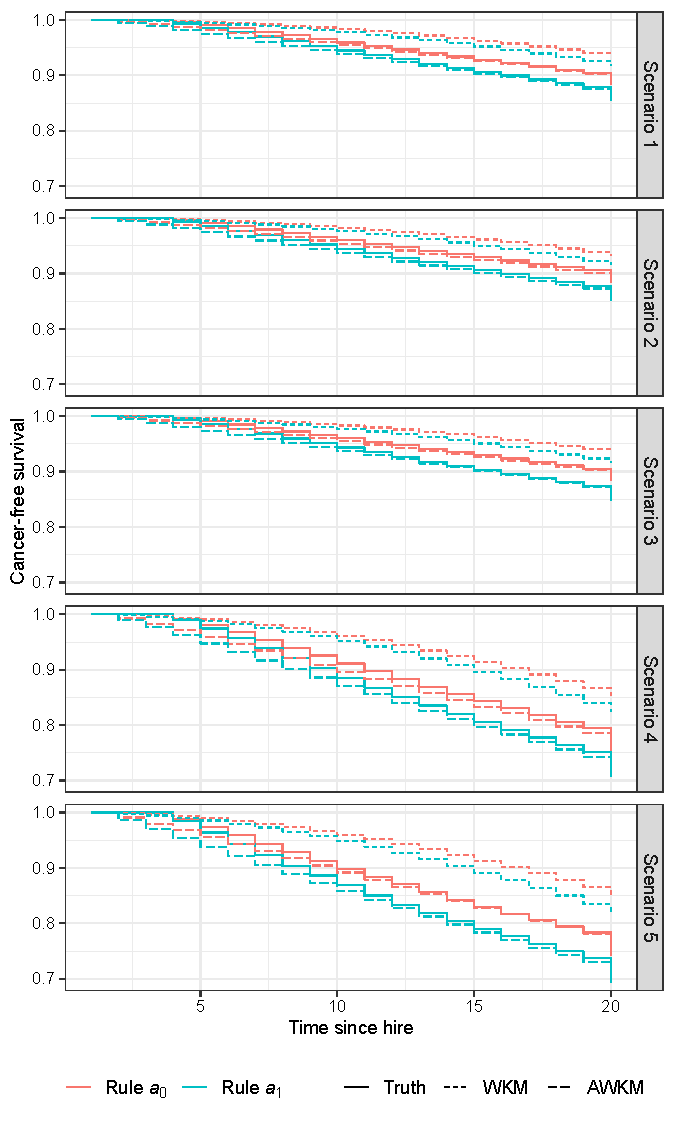
\includegraphics{/Users/kevinchen/Documents/2021 Fall/256 - Causal Inference/256-final/reports/resources/results.pdf}
\end{center}
\end{figure}

Table \ref{tab:survival} presents true and estimated average cancer-free
survival times under each intervention rule and scenario. Table
\ref{tab:differences} presents differences in survival time contrasting
rule \(a_1\) to rule \(a_0\). Table \ref{tab:bias} presents estimates of
the bias of the WKM and AWKM estimators for \(\psi\), the difference in
average cancer-free survival time over 20 years of follow-up. These
numeric results were consistent with the qualitative interpretations of
Figure \ref{fig:survival}. The WKM estimator over-estimated the
difference in cancer-free survival time, resulting in bias toward the
null, whereas the AWKM estimator under-estimates the cancer-free
survival, resulting in bias away from the null. In every scenario, the
bias of the WKM-derived contrast was two to several times larger in
magnitude than that of the AWKM-derived contrast.

The qualitative results here were consistent with those of Izano (2017).
However, true and estimated survival in the present analysis was larger
than those found previously. Furthermore, the true and estimator average
mean differences in survival were smaller in magnitude in the present
case. The magnitudes of the bias estimates were also smaller.

\begin{table}[H]
\centering
\caption{True cancer-free survival time $\mu_{a}$ over 20-year follow-up and estimator averages over 250 replicates.} 
\label{tab:survival}
\begin{tabular}{llrrrrr}
  \toprule
Rule & Estimator & Scenario 1 & Scenario 2 & Scenario 3 & Scenario 4 & Scenario 5 \\ 
  \midrule
$a_0$ & Truth & 19.08 & 19.10 & 19.10 & 18.02 & 17.83 \\ 
   & WKM & 19.52 & 19.51 & 19.52 & 18.91 & 18.90 \\ 
   & AWKM & 19.01 & 19.00 & 19.01 & 17.80 & 17.71 \\ 
   \midrule
$a_1$ & Truth & 18.80 & 18.79 & 18.76 & 17.54 & 17.29 \\ 
   & WKM & 19.41 & 19.39 & 19.39 & 18.68 & 18.67 \\ 
   & AWKM & 18.76 & 18.76 & 18.74 & 17.30 & 17.22 \\ 
   \bottomrule
\end{tabular}
\end{table}
\begin{table}[H]
\centering
\caption{Difference in average cancer-free survival time over 20-year follow-up comparing rule $a_1$ always exposed to rule $a_0$ never exposed at work: true value $\psi$ and estimator averages over 250 replicates.} 
\label{tab:differences}
\begin{tabular}{lrrrrr}
  \toprule
Estimator & Scenario 1 & Scenario 2 & Scenario 3 & Scenario 4 & Scenario 5 \\ 
  \midrule
Truth & -0.28 & -0.31 & -0.34 & -0.48 & -0.54 \\ 
  WKM & -0.11 & -0.12 & -0.13 & -0.23 & -0.23 \\ 
  AWKM & -0.25 & -0.24 & -0.27 & -0.50 & -0.50 \\ 
   \bottomrule
\end{tabular}
\end{table}
\begin{table}[H]
\centering
\caption{Bias estimates of estimators for $\psi$, the difference in average cancer-free survival time over 20 years of follow-up.} 
\label{tab:bias}
\begin{tabular}{lrrrrr}
  \toprule
Estimator & Scenario 1 & Scenario 2 & Scenario 3 & Scenario 4 & Scenario 5 \\ 
  \midrule
WKM & 0.17 & 0.19 & 0.21 & 0.25 & 0.31 \\ 
  AWKM & 0.03 & 0.07 & 0.07 & -0.02 & 0.04 \\ 
   \bottomrule
\end{tabular}
\end{table}

\hypertarget{application-to-the-uaw-gm-cohort}{%
\section{Application to the UAW-GM
Cohort}\label{application-to-the-uaw-gm-cohort}}

In the simulation study, we showed that under several scenarios
compatible with our hypothetical causal structure, the AWKM survival
estimator had a smaller bias than the WKM estimator. The bias was
smaller when the cumulative incidence of the outcome was low and at
later follow-up time points. Next, we estimated cancer-free survival in
a real-world context. Using data from two plants participating in the
UAW-GM Cohort study, we followed \(26\,182\) individuals starting from
hire to 35 years after hire for incidence of digestive system cancers
(colon, rectal, esophageal, or stomach). This duration of follow-up
spans a sizable proportion of a usual worker's working lifetime. As in
the simulation, the UAW-GM data were longitudinal data with baseline
covariates, time-varying covariates, and a survival outcome.

The exposures of interest were MWF of three types: straight, soluble,
and synthetic (Byers 2006; F. Mirer 2003; F. E. Mirer 2010). Straight
MWFs are hydrocarbon-based fluids that became widely-used by the 1920s.
They continue to occupy a large portion of the MWF market due to their
simple formulation. In straight MWFs, hydrocarbons of different lengths
are mixed together with other additives to attain different properties.
Straight MWFs contain polycyclic aromatic hydrocarbons, long known to be
carcinogenic (IARC 1973). Soluble oils are water-based oil emulsions
first introduced in response to rising oil prices. They now make up the
largest market share of MWFs (Childers 2006). Soluble MWFs are
vulnerable to microbial contamination, so they contain biocides and
chlorinated chemicals. Soluble MWFs have carcinogenic potential from
both their oil components and their additives, but their high lubricity
makes them the most popular fluid type. Synthetic MWFs have the best
toxicological profile, have no oil, and have a higher resistance to
microbial growth. They were introduced into the MWF market in the second
half of the 20th C., but failed to out-perform soluble MWFs in
industrial metalworking applications. Synthetic MWFs contain biocides,
corrosion inhibitors, and chlorinated compounds, some classified as
carcinogenic by the IARC (IARC 1987).

The outcome of interest was digestive system cancer incidence. There is
little past research linking digestive system cancers to MWF exposures,
but there is some evidence suggesting that straight MWFs cause digestive
system cancers (Izano et al. 2019). Cancer incidence was obtained by
linkage to Surveillance, Epidemiology, and End Results (SEER), which
recorded cancer incidence cases starting on January 1, 1973. The cohort
is comprised of individuals hired between 1938 and 1975. Cancer-free
survival to the start of the registry was a left-filtering process
possibly in the presence of the HWSE, as was the case in simulations.
Over the 35 year follow-up period, vital status was obtained through the
Social Security Administration, the National Death Index, as well as
records provided by the UAW. The exposure rules of interest in the
applied analysis were different than those in the simulation study:
\(a_0\) being exposed with 75\% chance in the years exposure was
observed and \(a_1\) being exposed in the years exposure was observed.
Weights were truncated at 1000. Exposure was binary and defined to be
whether there was exposure above the median level of exposure to
straight, soluble, and synthetic MWFs. Counterfactual survival under
rules \(a_0\) and \(a_1\) were estimated using the WKM and AWKM
estimators. Treatment and censoring mechanisms were estimated using
logistic regression conditional on baseline and time-varying
confounders. These logistic regressions were estimated with
stratification by every two years of follow-up. Baseline confounders
included race, sex, plant, and year of hire. Time-varying confounders
included age, cumulative time off, employment status, and exposure to
the metalworking fluids exposure from past years (3 years in the case of
exposure and 6 years in the case of death due to censoring). Summary
statistics for the full study population and those who experienced
digestive system cancer are presented in Table \ref{tab:popchar}.

\begin{table}[h]
\caption{Study population characteristics.}
\label{tab:popchar}
\begin{center}\begin{tabular}{lrlrl}
\toprule
&       \multicolumn{2}{c}{Full cohort}       & \multicolumn{2}{c}{Digestive cancer cases}      \\
\midrule
$n$ (person-years) 
                       &     26 182 & (695 475) & 213 & (6000) \\ 
Race (\%) \\
\hspace{1.5em} Black   &      6 017 & (23.0)  &  66 & (31.0)  \\ 
\hspace{1.5em} White   &     20 165 & (77.0)  & 147 & (69.0)  \\ 
Sex (\%) \\
\hspace{1.5em} Female  &      3 328 & (12.7)  &  15 & (7.0)  \\ 
\hspace{1.5em} Male    &     22 854 & (87.3)  & 198 & (93.0)  \\ 
Plant (\%) \\
\hspace{1.5em} Plant 1 &      9 092 & (34.7)  & 103 & (48.4)  \\ 
\hspace{1.5em} Plant 2 &     17 090 & (65.3)  & 110 & (51.6)  \\ 
\midrule
Ever exposed to MWF (\%)
                                            &      13 240 & (50.6)  &  95 & (44.6)  \\ 
Year of hire (mean (\textsc{sd}))
                                            &            1963 & (12.26) & 1960 & (9.55) \\ 
Age at end of follow-up (mean (\textsc{sd}))
                                            &         55.09 & (12.02) & 63.58 & (9.40) \\ 
Cumulative years off (mean (\textsc{sd}))
                                            &          0.06 & (0.15)  & 0.12 & (0.24)   \\
\bottomrule
\end{tabular}\end{center}
\end{table}

\hypertarget{assumptions}{%
\subsection{Assumptions}\label{assumptions}}

Since we are working with observational data, the evaluation of the
no-interference, causal consistency, ignorability, and overlap
(positivity) assumptions are critical for causal inference. The
stability of our estimation depends on positivity, which we assessed
qualitatively by examining the distribution of the weights. The
no-interference assumption may be problematized by the fact that there
were a finite number of job types in the factory setting. If one worker
operates a particular metalworking machine, then the the other workers
would not be able to operate that machine at that time. Instead, they
may be assigned to assembly tasks, which have lower MWF exposure
opportunities. That said, since these factories were quite large, there
may be approximate independence. The consistency assumption is also
problematic. The MWFs of interest are complex chemical mixtures whose
composition underwent changes by design and by nature of their use. Over
the last several decades, the formulation of MWFs has changed
significantly in reaction to performance needs and toxicity concerns (F.
Mirer 2003; Byers 2006). The composition of MWFs also undergoes
unintentional changes over the course of their use: MWFs are often
applied in contexts where contamination by other substances and microbes
is possible and chemical changes due to heat and pressure are likely. In
fact, concern over the carcinogenicity of MWFs includes concerns over
chemical species formed in MWF mixtures that were not originally added
(Hidajat et al. 2020). Concerns regarding the consistency assumption may
be abrogated in part by adequate adjustment for secular and
factory-level characteristics.

Another key assumption meriting discussion is that of sequential
ignorability. In order to achieve identification, even in the absence of
left filtering, we need to have conditionally ignorable future exposure
status and ignorable future censoring status at each time point given
past data. In occupational cohorts, employment status and health history
are strong predictors of future death (Häfner 1987; Halliday 2014;
Laliotis and Stavropoulou 2018). Logically, major causes of death first
act through employment status before they precipitate death. This
dynamic is actually a key component in the setup for HWSE. We are
therefore relatively confident that conditional ignorability of
censoring due to death is attained given covariate, exposure, and cancer
history. Our confidence in the conditional ignorability of exposure
given history was not as strong. In particular, workers may be assigned
to certain tasks based on their specific skills and knowledge, which may
be associated with structural privileges that confer a lower risk of
deleterious health outcomes. The potential magnitude of this
uncontrolled confounding may be bounded, however. Education level among
workers in the cohort was approximately homogeneous, and all cohort
members were members of the UAW union, which had uniform procedures in
place for equitable access to training, wages, and career advancement
(Harbison 1950; Barnard 2005). The presence of UAW policies support the
assertion that given time since hire, job types (and therefore
exposures) were randomly allocated.

\hypertarget{results-1}{%
\subsection{Results}\label{results-1}}

Estimated digestive system cancer-free curves under rules \(a_0\) and
\(a_1\) applied to the three MWF types are presented in Figure
\ref{fig:gm_survival}. Surprisingly, the survival curves were more or
less overlapping under the two exposure rules. Numeric values for the
cancer-free survival and difference in cancer-free survival are
presented in Tables \ref{tab:gm_survival} and \ref{tab:gm_differences}.
The numeric summaries were consistent with the qualitative
interpretation of the estimated survival curves; expected survival time
does not differ substantially comparing rules \(a_0\) and \(a_1\)
applied to all MWF types. Nonetheless, reducing exposure to straight and
soluble MWFs yielded a longer estimated survival time, though the
difference was less than a month in time.

\begin{figure}[h]
\caption{Cancer-free survival over time since hire under interventions for exposure to straight, soluble, and synthetic metalworking fluids. The estimated inverse probability weighted Kaplan-Meier (WKM) survival curve is represented by the solid. The estimated Aalen-filtered inverse probability weighted Kaplan-Meier (AWKM) survival curve is represented by the dashed-line. Salmon color indicates survival and survival estimates under rule $a_0$; cyan color indicates those under rule $a_1$.}
\label{fig:gm_survival}
\begin{center}
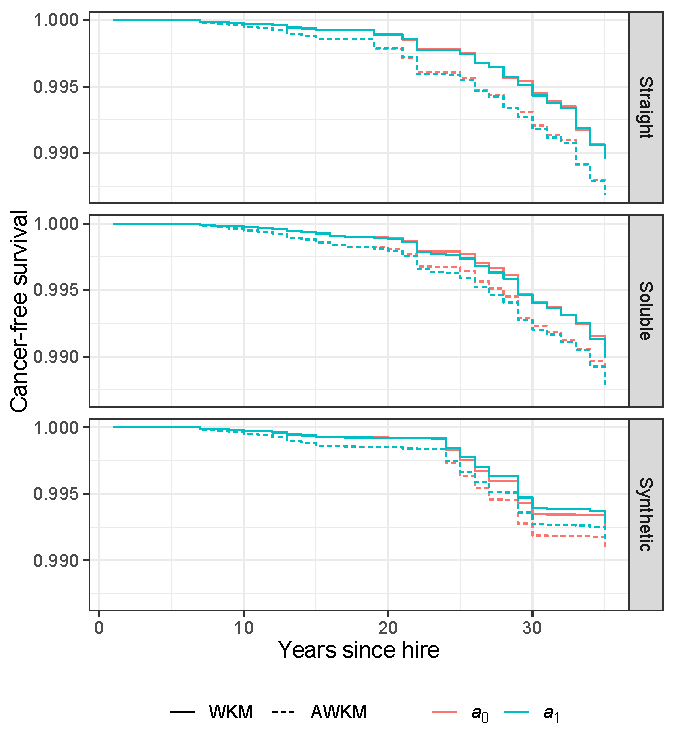
\includegraphics{/Users/kevinchen/Documents/2021 Fall/256 - Causal Inference/256-final/reports/resources/gm_results.pdf}
\end{center}
\end{figure}

\begin{table}[H]
\centering
\caption{Estimated cancer-free survival time over 35-year follow-up.} 
\label{tab:gm_survival}
\begin{tabular}{llrrr}
  \toprule
Rule & Estimator & Straight & Soluble & Synthetic \\ 
  \midrule
$a_0$ & WKM & 29.9606 & 29.9605 & 29.9626 \\ 
  $a_0$ & AWKM & 29.9337 & 29.9398 & 29.9443 \\ 
   \midrule
$a_1$ & WKM & 29.9600 & 29.9584 & 29.9648 \\ 
  $a_1$ & AWKM & 29.9325 & 29.9360 & 29.9479 \\ 
   \bottomrule
\end{tabular}
\end{table}
\begin{table}[H]
\centering
\caption{Estimated difference in average cancer-free survival time over 35-year follow-up comparing rule $a_1$ exposed above the median level of exposure with probability 1\% to $a_0$ never exposed.} 
\label{tab:gm_differences}
\begin{tabular}{lrrr}
  \toprule
Estimator & Straight & Soluble & Synthetic \\ 
  \midrule
WKM & -0.0006 & -0.0021 & 0.0022 \\ 
  AWKM & -0.0012 & -0.0039 & 0.0037 \\ 
   \bottomrule
\end{tabular}
\end{table}

Figure \ref{fig:gm_weights} presents the median cumulative weight
applied years since hire with ribbons showing the minimum and maximum
weight. The overlap in the distribution of weights under the two rules
for synthetic MWF exposure suggests that the model for the treatment and
censoring mechanisms were inadequate in distinguishing the units of
analysis by their probability of following a certain exposure rule or of
remaining alive. The distribution of the weights was very skewed.
Without truncation, they would have been in the order of magnitude of
\(10^{20}\) or even higher. Distributional summaries of the cumulative
weights without truncation are presented in Table \ref{tab:gm_w}. The
presence of extremely large weights suggests that our observed data were
inadequate for answering the causal questions of interest due to
practical violations in overlap (Petersen et al. 2012).

\begin{table}[H]
\centering
\caption{Summary statistics for the cumulative weights used for the WKM estimator at $t = 1$ and $t = 35$ years since hire for each metalworking fluid type and exposure rule.} 
\label{tab:gm_w}
\begin{tabular}{llrrrrrrr}
  \toprule
MWF type & Rule & $t$ & Minimum & Q1 & Median & Mean & Q3 & Maximum \\ 
  \midrule
Straight & $a_0$ &   1 & 1.00 & 1.00 & 1.00 &   1 & 1.00 &   1 \\ 
   & $a_1$ &   1 & 1.00 & 1.00 & 1.00 &   1 & 1.00 &   1 \\ 
  Soluble & $a_0$ &   1 & 1.00 & 1.00 & 1.00 &   1 & 1.00 &   1 \\ 
   & $a_1$ &   1 & 1.00 & 1.00 & 1.00 &   1 & 1.00 &   1 \\ 
  Synthetic & $a_0$ &   1 & 1.00 & 1.00 & 1.00 &   1 & 1.00 &   1 \\ 
   & $a_1$ &   1 & 1.00 & 1.00 & 1.00 &   1 & 1.00 &   1 \\ 
  Straight & $a_0$ &  35 & 0.00 & 2.25 & 4.71 & $9.7 \times 10^{16}$ & 4622.00 & $7.3 \times 10^{20}$ \\ 
   & $a_1$ &  35 & 0.00 & 2.70 & 13.40 & $1.3 \times 10^{18}$ & 22142.45 & $9.8 \times 10^{21}$ \\ 
  Soluble & $a_0$ &  35 & 0.00 & 4.04 & 858.96 & $5.2 \times 10^{15}$ & 74610.19 & $2.3 \times 10^{19}$ \\ 
   & $a_1$ &  35 & 0.00 & 158.56 & 6685.12 & $2.3 \times 10^{17}$ & 1227858.13 & $1.7 \times 10^{21}$ \\ 
  Synthetic & $a_0$ &  35 & 0.00 & 1.02 & 1.25 & $3.7 \times 10^{19}$ & 8.85 & $3.2 \times 10^{23}$ \\ 
   & $a_1$ &  35 & 0.00 & 1.02 & 1.36 & $2.1 \times 10^{21}$ & 22.63 & $1.8 \times 10^{25}$ \\ 
   \bottomrule
\end{tabular}
\end{table}

\begin{figure}
\caption{Median of the cumulative weights for each year since hire with ribbons delimiting the range of values calculated. Salmon color corresponds to the weights used in the estimation of the survival curve under rule $a_0$; cyan corresponds to those for rule $a_1$.}
\label{fig:gm_weights}
\begin{center}
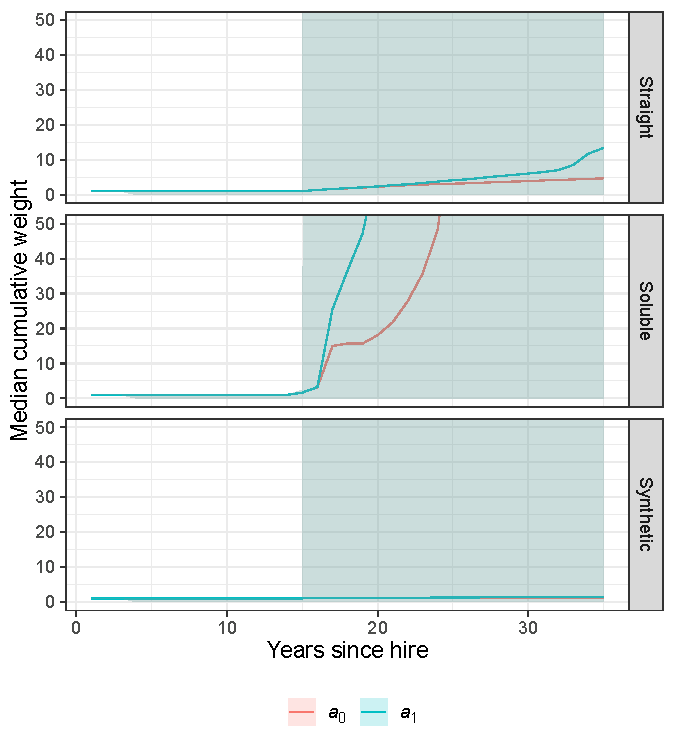
\includegraphics{/Users/kevinchen/Documents/2021 Fall/256 - Causal Inference/256-final/reports/resources/gm_weights.pdf}
\end{center}
\end{figure}

\hypertarget{discussion}{%
\section{Discussion}\label{discussion}}

In the simulation study, we showed that the inverse probability of
exposure/censoring weighted Kaplan-Meier estimator resulted in lower
bias in the estimation of average survival time than did the weighted
Kaplan-Meier estimator without the Aalen filter. While the Aalen filter
corrects for non-informative left-filtering in the estimation of the
discrete hazard by excluding person-years not observed under the cancer
registry. These person-years contribute to estimation during the
estimation of exposure and censoring weights. Speculatively, the
combination of the two extensions to the Kaplan-Meier estimator may
result in the partial control of informative left censoring without
adjusting for informative left truncation.

The simulation permitted the evaluation of the estimators in clean,
well-behaved scenarios, but the same luxury was not possible when using
observed data. Several assumptions used in the simulation study were
incompatible with what is known about cancer etiology. Firstly,
cumulative incidence in the simulations was close to 15\% (or higher)
over a 20-year follow-up. This is an extraordinarily high risk of
cancer, especially because most workers in the automotive manufacturing
industry start their careers at a fairly young age. Digestive system
cancers are among the most common forms of cancer in the Unite states,
but over 35 years of follow-up, we were only able to observe a
cumulative incidence of less than 1\%. The simulation results suggested
that the bias of the WKM and AWKM estimators is higher when cumulative
incidence is higher, but when cumulative incidence is low, there is a
different problem: the reliance on few observations to index the risk
sets.

There are multiple opportunities for future work. The simulation study
can be expanded to investigate subtler exposure-outcome effects. In the
present work, the discrete hazard ratio of cancer incidence given
exposure was rather high at about 1.28. Furthermore, we assumed the
luxury of knowing the true treatment and censoring mechanisms' model
forms, but this is quite unrealistic. In future simulations, the effect
of model mis-specification should be investigated. Alternatively, we
could estimate survival using a doubly robust method. There can also be
several improvements made from the subject-matter expertise
point-of-view. The exposure rules investigated in the applied analysis
were chosen naively. Other dynamic or stochastic exposure interventions
may have been of greater interest to occupational health policy, and
they may have led to improved numeric performance as well. The present
analysis did not lag exposure status, which is standard practice in
cancer epidemiology -- the biological responses to carcinogens do not
occur until several years or decades after exposure. The true causal
effects of MWF exposure may not yet be observable after 35 years of
follow-up. As follow-up in this cohort study continues, we will have the
opportunity to investigate the carcinogenic effects of MWF exposure
further.

\newpage

\hypertarget{references}{%
\section*{References}\label{references}}
\addcontentsline{toc}{section}{References}

\hypertarget{refs}{}
\begin{CSLReferences}{1}{0}
\leavevmode\hypertarget{ref-Andersen_1993}{}%
Andersen, P. K., Ø. Borgan, R. D. Gill, and N. Keiding. 1993.
\emph{Statistical Models Based on Counting Processes}. Springer Series
in Statistics. Springer, New York, NY.
\url{https://books.google.com/books?id=kBnvAAAAMAAJ}.

\leavevmode\hypertarget{ref-Arrighi_1994}{}%
Arrighi, H. Michael, and Irva Hertz-Picciotto. 1994. {``The Evolving
Concept of the Healthy Worker Survivor Effect.''} \emph{Epidemiology} 5
(2): 189--96. \url{http://www.jstor.org/stable/3702361}.

\leavevmode\hypertarget{ref-Barnard_2005}{}%
Barnard, John. 2005. \emph{American Vanguard: The United Auto Workers
During the Reuther Years, 1935-1970}. Wayne State University Press.

\leavevmode\hypertarget{ref-Byers_2006}{}%
Byers, Jerry P. 2006. \emph{Metalworking Fluids}. CRC Press.

\leavevmode\hypertarget{ref-Childers_2006}{}%
Childers, Jean. 2006. {``The Chemistry of Metalworking Fluids.''} In
\emph{Metalworking Fluids}. CRC Press.

\leavevmode\hypertarget{ref-Eisen_2001}{}%
Eisen, Ellen A, Judith Bardin, Rebecca Gore, Susan R Woskie, Marilyn F
Hallock, and Richard R Monson. 2001. {``Exposure-Response Models Based
on Extended Follow-up of a Cohort Mortality Study in the Automobile
Industry.''} \emph{Scandinavian Journal of Work, Environment \& Health}
27 (4): 240--49.

\leavevmode\hypertarget{ref-Eisen_1992}{}%
Eisen, Ellen A, Paige E Tolbert, Richard R Monson, and Thomas J Smith.
1992. {``Mortality Studies of Machining Fluid Exposure in the Automobile
Industry {I}: A Standardized Mortality Ratio Analysis.''} \emph{American
Journal of Industrial Medicine} 22 (6): 809--24.

\leavevmode\hypertarget{ref-Frangakis_2002}{}%
Frangakis, Constantine E, and Donald B Rubin. 2002. {``Principal
Stratification in Causal Inference.''} \emph{Biometrics} 58 (1): 21--29.

\leavevmode\hypertarget{ref-Garcia_2017}{}%
Garcia, Erika, Sally Picciotto, Sadie Costello, Patrick T Bradshaw, and
Ellen A Eisen. 2017. {``Assessment of the Healthy Worker Survivor Effect
in Cancer Studies of the United Autoworkers-General Motors Cohort.''}
\emph{Occupational and Environmental Medicine} 74 (4): 294--300.

\leavevmode\hypertarget{ref-Garcia_2018}{}%
Garcia, Erika, Sally Picciotto, Andreas M Neophytou, Patrick T Bradshaw,
John R Balmes, and Ellen A Eisen. 2018. {``Lung Cancer Mortality and
Exposure to Synthetic Metalworking Fluid and Biocides: Controlling for
the Healthy Worker Survivor Effect.''} \emph{Occupational and
Environmental Medicine} 75 (10): 730--35.

\leavevmode\hypertarget{ref-Halliday_2014}{}%
Halliday, Timothy J. 2014. {``Unemployment and Mortality: Evidence from
the PSID.''} \emph{Soc Sci Med} 113 (July): 15--22.
\url{https://doi.org/10.1016/j.socscimed.2014.04.038}.

\leavevmode\hypertarget{ref-Harbison_1950}{}%
Harbison, Frederick H. 1950. {``The General Motors-United Auto Workers
Agreement of 1950.''} \emph{Journal of Political Economy} 58 (5):
397--411.

\leavevmode\hypertarget{ref-Hafner_1987}{}%
Häfner, H. 1987. {``Unemployment and Health.''} \emph{Dtsch Med
Wochenschr} 112 (37): 1428--32.
\url{https://doi.org/10.1055/s-2008-1068265}.

\leavevmode\hypertarget{ref-Hidajat_2020}{}%
Hidajat, Mira, Damien Martin McElvenny, Peter Ritchie, Andrew Darnton,
William Mueller, Raymond M Agius, John W Cherrie, and Frank de Vocht.
2020. {``Lifetime Cumulative Exposure to Rubber Dust, Fumes and
n-Nitrosamines and Non-Cancer Mortality: A 49-Year Follow-up of UK
Rubber Factory Workers.''} \emph{Occup Environ Med} 77 (5): 316--23.
\url{https://doi.org/10.1136/oemed-2019-106269}.

\leavevmode\hypertarget{ref-IARC_1973}{}%
IARC. 1973. \emph{IARC Monographs on the Evaluation of Carcinogenic Risk
of the Chemical to Man: Certain Polycyclic Aromatic Hydrocarbons and
Heterocyclic Compounds}. Vol. 3. World Health Organization International
Agency for Research on Cancer.

\leavevmode\hypertarget{ref-IARC_1987}{}%
---------. 1987. \emph{IARC Monographs on the Evaluation of the
Carcinogenic Risk of Chemicals to Humans. Overall Evaluations of
Carcinogenicity: An Updating of IARC Monographs, Volumes 1 to 42}.
\emph{World Health Organization}. Vol. 7. World Health Organization
International Agency for Research on Cancer.

\leavevmode\hypertarget{ref-Izano_2017_thesis}{}%
Izano, Monika A. 2017. {``Estimating Causal Effects of Occupational
Exposures.''} PhD thesis, University of California, Berkeley; University
of California, Berkeley.

\leavevmode\hypertarget{ref-Izano_2019}{}%
Izano, Monika A, Oleg A Sofrygin, Sally Picciotto, Patrick T Bradshaw,
and Ellen A Eisen. 2019. {``Metalworking Fluids and Colon Cancer Risk:
Longitudinal Targeted Minimum Loss-Based Estimation.''}
\emph{Environmental Epidemiology} 3 (1): e035.

\leavevmode\hypertarget{ref-Kaplan_1958}{}%
Kaplan, Edward L, and Paul Meier. 1958. {``Nonparametric Estimation from
Incomplete Observations.''} \emph{Journal of the American Statistical
Association} 53 (282): 457--81.

\leavevmode\hypertarget{ref-Laliotis_2018}{}%
Laliotis, Ioannis, and Charitini Stavropoulou. 2018. {``Crises and
Mortality: Does the Level of Unemployment Matter?''} \emph{Soc Sci Med}
214 (October): 99--109.
\url{https://doi.org/10.1016/j.socscimed.2018.08.016}.

\leavevmode\hypertarget{ref-Mirer_2003}{}%
Mirer, Franklin. 2003. {``Updated Epidemiology of Workers Exposed to
Metalworking Fluids Provides Sufficient Evidence for Carcinogenicity.''}
\emph{Applied Occupational and Environmental Hygiene} 18 (11): 902--12.

\leavevmode\hypertarget{ref-Mirer_2010}{}%
Mirer, Franklin E. 2010. {``New Evidence on the Health Hazards and
Control of Metalworking Fluids Since Completion of the OSHA Advisory
Committee Report.''} \emph{American Journal of Industrial Medicine} 53
(8): 792--801.

\leavevmode\hypertarget{ref-Naimi_2013}{}%
Naimi, Ashley I, Stephen R Cole, Michael G Hudgens, M Alan Brookhart,
and David B Richardson. 2013. {``Assessing the Component Associations of
the Healthy Worker Survivor Bias: Occupational Asbestos Exposure and
Lung Cancer Mortality.''} \emph{Annals of Epidemiology} 23 (6): 334--41.

\leavevmode\hypertarget{ref-Pearl_1995}{}%
Pearl, Judea. 1995. {``Causal Diagrams for Empirical Research.''}
\emph{Biometrika} 82 (4): 669--88.

\leavevmode\hypertarget{ref-Petersen_2012}{}%
Petersen, Maya L, Kristin E Porter, Susan Gruber, Yue Wang, and Mark J
van der Laan. 2012. {``Diagnosing and Responding to Violations in the
Positivity Assumption.''} \emph{Statistical Methods in Medical Research}
21 (1): 31--54. \url{https://doi.org/10.1177/0962280210386207}.

\leavevmode\hypertarget{ref-Sofrygin_2021}{}%
Sofrygin, Oleg, Mark J. van der Laan, and Romain Neugebauer. 2021.
\emph{Stremr: Streamlined Estimation for Static, Dynamic and Stochastic
Treatment Regimes in Longitudinal Data}.
\url{https://github.com/osofr/stremr}.

\leavevmode\hypertarget{ref-Xie_2005}{}%
Xie, Jun, and Chaofeng Liu. 2005. {``Adjusted Kaplan--Meier Estimator
and Log-Rank Test with Inverse Probability of Treatment Weighting for
Survival Data.''} \emph{Statistics in Medicine} 24 (20): 3089--3110.

\end{CSLReferences}

\end{document}
